\documentclass{scrreprt}
\usepackage{amsmath}
\usepackage{listings}
\usepackage{array}
\usepackage{amsmath}
\usepackage[a4paper, margin=1in]{geometry}
\usepackage{tikz} 
\usepackage{underscore}
\usepackage[bookmarks=true]{hyperref}
\usepackage[utf8]{inputenc}
\usepackage[english]{babel}
\usepackage{enumitem}
\usepackage[a4paper, margin=1in]{geometry}
\usetikzlibrary{shapes, arrows.meta, positioning, backgrounds}

% Define styles for different node types
\tikzstyle{startstop} = [rectangle, rounded corners, minimum width=3cm, minimum height=1cm, text centered, draw=black, fill=red!30]
\tikzstyle{process} = [rectangle, minimum width=3.5cm, minimum height=1cm, text centered, draw=black, fill=blue!30]
\tikzstyle{arrow} = [thick,->,>=stealth]

% Define stickman style
\tikzset{
    stickman/.pic={
        % Head
        \draw[fill=gray] (0,0.6) circle (0.3cm);
        % Body
        \draw[line width=0.5mm] (0,0.3) -- (0,-0.6);
        % Arms
        \draw[line width=0.5mm] (-0.4,0.3) -- (0.4,0.3);
        % Legs
        \draw[line width=0.5mm] (0,-0.6) -- (-0.4,-1.2);
        \draw[line width=0.5mm] (0,-0.6) -- (0.4,-1.2);
    }
}

% Hyperref settings
\hypersetup{
    pdftitle={Software Requirement Specification},
    pdfauthor={Jean-Philippe Eisenbarth},
    pdfsubject={TeX and LaTeX},
    pdfkeywords={TeX, LaTeX, graphics, images},
    colorlinks=true,
    linkcolor=blue,
    citecolor=black,
    filecolor=black,
    urlcolor=purple,
    linktoc=page
}

% Set extra row height and padding
\setlength{\extrarowheight}{4pt}
\renewcommand{\arraystretch}{1.5}

\begin{document}

\begin{titlepage}
    \centering
    \includegraphics[width=0.5\textwidth]{./logo.png} 
    \vspace{1cm}

    \textbf{Department of Computer Science and Engineering}\\
    Premier University
    \vspace{1cm}

     \large \textnormal{CSE 302 : Computational Methods for Engineering 
    Problems Laboratory }
    \vspace{1in} 

    \Large \textnormal{Title: Implementation of Bisection, Falsi, and Newton-Raphson Methods for Root Finding}
    \vspace{0.5in} 

    \large
    \textbf{Submitted by:}
    \vspace{0.5cm}

    \renewcommand{\arraystretch}{1.5} 
    \begin{tabular}{|p{0.4\textwidth}|p{0.6\textwidth}|}
        \hline
        \textbf{Name} & Mohammad Hafizur Rahman Sakib \\ 
        \hline
        \textbf{ID} & 0222210005101118 \\ 
        \hline
        \textbf{chapter} & C \\ 
        \hline
        \textbf{Session} & Spring 2024 \\ 
        \hline
        \textbf{Semester} & 5th Semester \\ 
        \hline
        \textbf{Submission Date} & 14.09.2024 \\ 
        \hline
    \end{tabular}
    \vspace{1cm}

    \begin{minipage}[t]{0.48\textwidth}
        \textbf{Submitted to:}\\
        Kollol Dey\\
        Lecturer, Department of EEE\\
        Premier University\\
        Chittagong
    \end{minipage}% 
    \hfill 
    \begin{minipage}[t]{0.48\textwidth}
        \raggedleft
        \textbf{Remarks}\\
        \vspace{0.5cm} % Adjust vertical space for remarks
        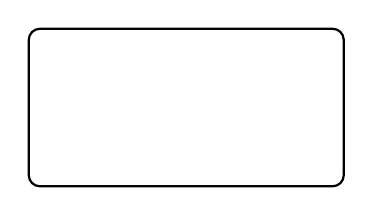
\begin{tikzpicture}
            \draw[thick, rounded corners] (0,0) rectangle (4,2);
        \end{tikzpicture}
    \end{minipage}

    \date{\today}
    \vfill
\end{titlepage}

\section*{Introduction}
This report presents the implementation and output of three widely used root-finding methods: the Bisection method, the False Position (Falsi) method, and the Newton-Raphson method. Each method is applied to solve a given mathematical equation, and the code along with its output is provided. The goal is to demonstrate how each algorithm approaches root finding without comparing their efficiencies or convergence rates.

\section*{Bisection Method}

The Bisection method is an iterative technique for finding the root of a function by repeatedly dividing an interval in half and selecting the subinterval where the root lies.

\subsection*{Formula}

Given a function \( f(x) \) and an interval \([a, b]\) where \( f(a) \) and \( f(b) \) have opposite signs, the next approximation \( x_{n+1} \) is calculated using:

\begin{equation}
x_{n+1} = \frac{a + b}{2}
\end{equation}

where:
- \( a \) and \( b \) are the current interval bounds.

\subsection*{Steps}

\begin{enumerate}
    \item Choose an initial interval \([a, b]\) such that \( f(a) \) and \( f(b) \) have opposite signs.
    \item Compute the midpoint \( x_{n+1} \) using:
    \begin{equation}
    x_{n+1} = \frac{a + b}{2}
    \end{equation}
    \item Determine the subinterval \([a, x_{n+1}]\) or \([x_{n+1}, b]\) where the function changes sign.
    \item Repeat until the interval size \( |b - a| \) is smaller than a predefined tolerance.
\end{enumerate}

\subsection*{Advantages}

\begin{itemize}
    \item Guarantees convergence if the initial interval contains a root.
    \item Simple and easy to implement.
\end{itemize}

\subsection*{Limitations}

\begin{itemize}
    \item Can be slow to converge compared to other methods.
    \item Requires the function to be continuous.
\end{itemize}

\subsection*{Source Code : }
\begin{center}
    {\includegraphics[width=350px, height=520px]{bisection_code.png}}
    \parbox{0.8\textwidth}{ 
        \centering
        \textbf{Figure : Source Code for Bisection Method}
    }
\end{center}
\newpage
\subsection*{Output : }
\begin{center}
    {\includegraphics[width=500px, height=320px]{bisection_output.png}}
    \parbox{0.8\textwidth}{ 
        \centering
        \textbf{Figure : Output for Bisection Method}
    }
\end{center}
\section*{False Position (Falsi) Method}

The False Position method is an iterative technique for finding the roots of a function. It improves on the Bisection method by using a secant line to estimate the root.

\subsection*{Formula}

Given a function \( f(x) \), the next approximation \( x_{n+1} \) is calculated using:

\begin{equation}
x_{n+1} = x_n - \frac{f(x_n) \cdot (x_u - x_n)}{f(x_u) - f(x_n)}
\end{equation}

where:
- \( x_n \) is the current approximation.
- \( x_u \) is the upper bound of the interval.

\subsection*{Steps}

\begin{enumerate}
    \item Choose initial guesses \( x_l \) and \( x_u \) such that \( f(x_l) \) and \( f(x_u) \) have opposite signs.
    \item Compute the next approximation using:
    \begin{equation}
    x_{n+1} = x_n - \frac{f(x_n) \cdot (x_u - x_n)}{f(x_u) - f(x_n)}
    \end{equation}
    \item Update the interval based on the sign of \( f(x_{n+1}) \).
    \item Repeat until the difference \( |x_{n+1} - x_n| \) is smaller than a predefined tolerance.
\end{enumerate}

\subsection*{Advantages}

\begin{itemize}
    \item Faster convergence than the Bisection method.
    \item Does not require derivative information.
\end{itemize}

\subsection*{Limitations}

\begin{itemize}
    \item May converge slowly if the function is not well-behaved.
    \item Requires an initial interval with a sign change.
\end{itemize}


\subsection*{Source Code : }
\begin{center}
    {\includegraphics[width=350px, height=500px]{falsi_code.png}}
    \parbox{0.8\textwidth}{ 
        \centering
        \textbf{Figure : Source Code for Falsi Method}
    }
\newpage
\end{center}
\subsection*{Output : }
\begin{center}
    {\includegraphics[width=475px, height=180px]{falsi_output1.png}}
    \parbox{0.8\textwidth}{ 
        \centering
        \textbf{Figure : Output for Falsi Method}
    }
\end{center}

\section*{Newton-Raphson Method}

The Newton-Raphson method is an iterative technique for approximating the roots of a function. It uses the function's derivative to refine guesses for the root.

\subsection*{Formula}

Given a function \( f(x) \) and its derivative \( f'(x) \), the iteration formula is:

\begin{equation}
x_{n+1} = x_n - \frac{f(x_n)}{f'(x_n)}
\end{equation}

\subsection*{Steps}

\begin{enumerate}
    \item Start with an initial guess \( x_0 \).
    \item Update the guess using:
    \begin{equation}
    x_{n+1} = x_n - \frac{f(x_n)}{f'(x_n)}
    \end{equation}
    \item Repeat until \( |x_{n+1} - x_n| \) is smaller than a predefined tolerance.
\end{enumerate}

\subsection*{Advantages}

\begin{itemize}
    \item Fast convergence near the root.
    \item Simple to implement.
\end{itemize}

\subsection*{Limitations}

\begin{itemize}
    \item Requires a good initial guess.
    \item Needs the derivative of the function.
\end{itemize}

\subsection*{Source Code : }
\begin{center}
    {\includegraphics[width=350px, height=420px]{newton_code.png}}
    \parbox{0.8\textwidth}{ 
        \centering
        \textbf{Figure : Source Code for Newton Raphson Method}
    }
\end{center}
\subsection*{Output : }
\begin{center}
    {\includegraphics[width=475px, height=180px]{newton_output.png}}
    \parbox{0.8\textwidth}{ 
        \centering
        \textbf{Figure : Output for Newton Raphson Method}
    }
\end{center}

\section*{Conclusion}

In this report, we have demonstrated the implementation of three root-finding methods: the Bisection method, the False Position (Falsi) method, and the Newton-Raphson method. Each method offers a unique approach to approximating the roots of a function:

\begin{itemize}
    \item The Bisection method provides a reliable but slower approach by iteratively narrowing down an interval where the root lies.
    \item The False Position method improves upon the Bisection method by using a secant line to enhance convergence speed while still requiring an interval with a sign change.
    \item The Newton-Raphson method offers rapid convergence near the root by using the function's derivative, though it depends on a good initial guess and the availability of the derivative.
\end{itemize}

The provided code and outputs illustrate the practical application of these methods, showcasing their ability to find roots effectively. While the Bisection and False Position methods are useful for their simplicity and reliability, the Newton-Raphson method stands out for its efficiency in converging to the root under suitable conditions.

Overall, this report highlights the versatility of these root-finding techniques and their applicability in solving mathematical equations. Each method has its advantages and limitations, making them suitable for different scenarios based on the problem's requirements and characteristics.


\end{document}
